\documentclass[border=10pt]{standalone}
\usepackage{tikz}
\usetikzlibrary{shapes.multipart, positioning, arrows.meta, shadows, calc}

\definecolor{HeaderColor}{RGB}{0, 51, 102}      % Navy Blue
\definecolor{BgColor}{RGB}{245, 245, 255}       % Very light blue/white
\definecolor{LineColor}{RGB}{50, 50, 50}        % Dark Gray

% Define entity style
\tikzset{
    entity/.style={
        draw=HeaderColor, 
        thick, 
        rectangle split, 
        rectangle split parts=2,
        rectangle split part fill={HeaderColor, BgColor},
        align=left, 
        font=\small, 
        rounded corners=3pt,
        text width=4.5cm,
        inner sep=4pt
    }
}

\begin{document}
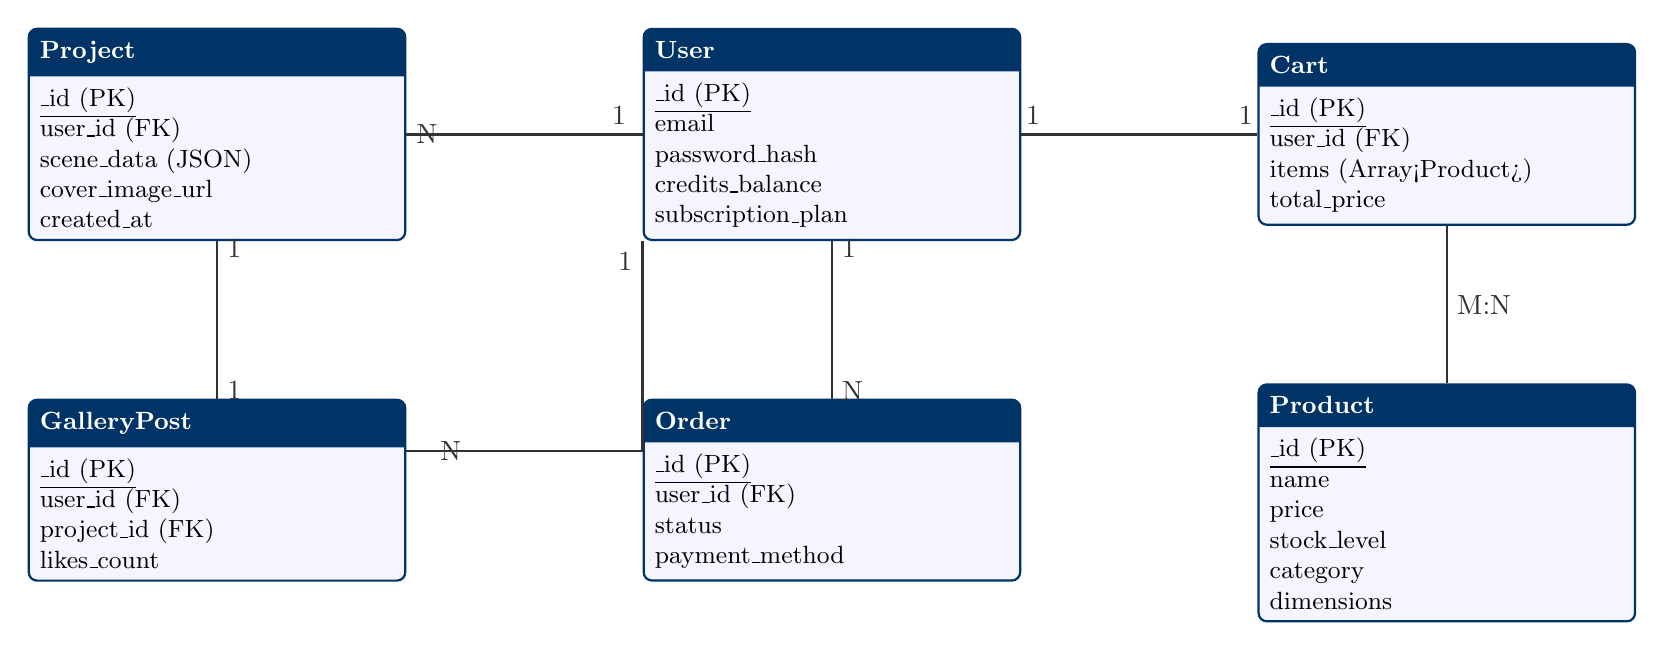
\begin{tikzpicture}[node distance=2.5cm, every text node part/.style={align=left}]

    % ============================================================================
    % ENTITIES
    % ============================================================================

    % Central Entity: User
    \node[entity] (User) {
        \textcolor{white}{\textbf{User}}
        \nodepart{two}
        \underline{\_id (PK)} \\
        email \\
        password\_hash \\
        credits\_balance \\
        subscription\_plan
    };

    % Left Side: Project
    \node[entity, left=3cm of User] (Project) {
        \textcolor{white}{\textbf{Project}}
        \nodepart{two}
        \underline{\_id (PK)} \\
        user\_id (FK) \\
        scene\_data (JSON) \\
        cover\_image\_url \\
        created\_at
    };

    % Bottom Left: GalleryPost
    \node[entity, below=2cm of Project] (GalleryPost) {
        \textcolor{white}{\textbf{GalleryPost}}
        \nodepart{two}
        \underline{\_id (PK)} \\
        user\_id (FK) \\
        project\_id (FK) \\
        likes\_count
    };

    % Right Side: Cart
    \node[entity, right=3cm of User] (Cart) {
        \textcolor{white}{\textbf{Cart}}
        \nodepart{two}
        \underline{\_id (PK)} \\
        user\_id (FK) \\
        items (Array<Product>) \\
        total\_price
    };

    % Far Right: Product
    \node[entity, below=2cm of Cart] (Product) {
        \textcolor{white}{\textbf{Product}}
        \nodepart{two}
        \underline{\_id (PK)} \\
        name \\
        price \\
        stock\_level \\
        category \\
        dimensions
    };

    % Bottom: Order
    \node[entity, below=2cm of User] (Order) {
        \textcolor{white}{\textbf{Order}}
        \nodepart{two}
        \underline{\_id (PK)} \\
        user\_id (FK) \\
        status \\
        payment\_method
    };

    % ============================================================================
    % RELATIONSHIPS
    % ============================================================================

    % Style for relationship lines
    \tikzset{
        rel/.style={
            draw=LineColor, 
            thick, 
            -{Circle[open] . Straight Barb[angle=60:3mm]}, % Crow's foot ish look on one end
        },
        one/.style={
            -{Bar[width=3mm] . Bar[width=3mm]}
        }
    }

    % User (1) to Project (N)
    \draw[thick, LineColor] (User.west) -| node[pos=0.05, above] {1} node[pos=0.95, right] {N} (Project.east);

    % User (1) to Order (N)
    \draw[thick, LineColor] (User.south) -- node[pos=0.05, right] {1} node[pos=0.95, right] {N} (Order.north);

    % User (1) to Cart (1)
    \draw[thick, LineColor] (User.east) -- node[pos=0.05, above] {1} node[pos=0.95, above] {1} (Cart.west);

    % User (1) to GalleryPost (N)
    % Routing via orthogonal lines to avoid crossing User-Order line badly
    \draw[thick, LineColor] (User.south west) |- node[pos=0.05, left] {1} node[pos=0.95, right] {N} ($(GalleryPost.east) + (0, 0.5)$);

    % Project (1) to GalleryPost (1 or N? Usually 1 post per project reference)
    % Assuming Project can be shared once, or multiple times. Let's link them.
    \draw[thick, LineColor] (Project.south) -- node[pos=0.05, right] {1} node[pos=0.95, right] {1} (GalleryPost.north);

    % Cart (M) to Product (N)
    \draw[thick, LineColor] (Cart.south) -- node[pos=0.5, right] {M:N} (Product.north);
    
    % Relationship Decoration (Optional Crow's Foot Emulation with labels)
    
\end{tikzpicture}
\end{document}
